\subsection{
    Преобразование матрицы линейного оператора при переходе к новому базису (вывести формулу).
}

\begin{theorem}
    Матрицы $A_b$ и $A_e$ линейного оператора $\mathscr{A} \colon \mathcal{L} \to \mathcal{L}$, записанные в базисах $b$ и $e$ линейного пространства $\mathcal{L}$, связаны друг с другом соотношением
    
    $$A_e = T^{-1}_{b \to e}A_bT_{b \to e}.$$
\end{theorem}

\begin{proof}~

    Пусть $\vec{y} = \mathscr{A}\vec{x}$. Обозначим координаты векторов $\vec{x}$ и $\vec{y}$ в старом базисе $b$ через $x_b$ и $y_b$, а в новом базисе $e$ - через $x_e$ и $y_e$. Поскольку действие линейного оператора $\mathscr{A}$ в матричной форме в базисе $b$ имеет вид $y_b = A_bx_b$ (\textbf{*}см. теорему \ref{thm:theorem_21_1}), а координаты векторов $\vec{x}$ и $\vec{y}$ в новом и старом базисах связаны между собой равенствами (\textbf{*}см. билет 17.)

    $$x_b = T_{b \to e}x_e, \quad \quad y_b = T_{b \to e}y_e,$$

    то получаем

    $$y_e = T^{-1}_{b \to e}y_b = T^{-1}_{b \to e}(A_bx_b) = T^{-1}_{b \to e}(A_bT_{b \to e}x_e) = (T^{-1}_{b \to e}A_bT_{b \to e})x_e.$$
    Равенство $y_e = (T^{-1}_{b \to e}A_bT_{b \to e})x_e$ является матричной формой записи действия линейного оператора $\mathscr{A}$ в базисе $e$ и поэтому, согласно теореме \ref{thm:theorem_21_1}, $T^{-1}_{b \to e}A_bT_{b \to e} = A_e$. 

    Изложенное доказательство теоремы хорошо иллюстрирует следующая диаграмма:

    \begin{figure}[H]
        \centering
        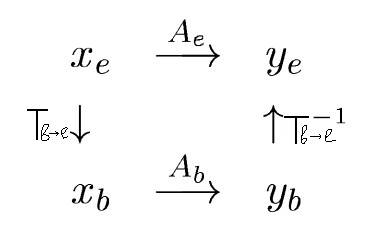
\includegraphics[scale=0.5]{images/module2/question22/1.jpg}
        \label{fig:picture_22_1}
    \end{figure}
\end{proof}
